\title{Covariant Phase Space via MultiSymplectic Geometry}
\author{
        Antonio Michele Miti \\
                Department of Mathematics and Physics\\
        Università Cattolica del Sacro Cuore\\
        via Musei X, Brescia xxx, \underline{Italy}
}
\date{\today}

\documentclass[12pt]{article}

\usepackage{amsmath}
\usepackage[diffgeo]{../Math-Symbols-List/commonmathsymb}
\usepackage{standalone}


\begin{document}
\maketitle

\begin{abstract}
This is the paper's abstract \ldots
\end{abstract}

\section{Introduction: multisymplectic landscape at glance}
Let's briefly recall in what consists the multisymplectic approach to mechanics of field systems in order to understand its relationship with the covariant phase space approach.

\begin{figure}
  \centering
  \includestandalone[mode=buildnew]{ms_landscape}
  \caption{interesting results}
\end{figure}

\begin{itemize}
 \item the starting point is the \emph{configuration bundle} 
 	\begin{displaymath}
 		E = \left( \pi_{M,E} : E\rightarrow M \right)
 	\end{displaymath}
 	the object encoding the kinematics.
 \item from that we have constructed the \emph{I jet bundle} applying the jet functor to $E$ 
 	\begin{displaymath}
 	J^1E = \left( \pi_{J^1 M,E} : J^1 M\rightarrow M \right)
 	\end{displaymath} 
 	that is an affine bundle over $E$.
 \item Then, we considered other two vector bundle derived from the first jet:
 	\begin{displaymath}
 	J^{1 \TwistedAffine}E = \left( \pi_{J^{1 \TwistedAffine} M,E} : J^{1 \TwistedAffine} M\rightarrow M \right)
 	\end{displaymath}
	twisted affine dual of $J^1E$ called \emph{"extended multiphase space"}.
	\begin{displaymath}
	\vec{J}^{1 \TwistedLinear}E = \left( \pi_{J^{1 \TwistedLinear} M,E} : J^{1 \TwistedLinear} M\rightarrow M \right)
	\end{displaymath}
	twisted linear dual of $J^1 E$ called \emph{"standard multiphase space"}. \footnote{It can be seen as the dual bundle of the vector bundle $\vec{J^1E}$ linear model of $J^1E$}
	The first one can be also seen as an affine line bundle over the second one.


\end{itemize}

\paragraph{Outline}
The remainder of this article is organized as follows.
Section~\ref{previous work} gives account of previous work.
Our new and exciting results are described in Section~\ref{results}.
Finally, Section~\ref{conclusions} gives the conclusions.

\section{Previous work}\label{previous work}
\begin{figure}
  \centering
  \includestandalone[mode=buildnew]{ms_sigmaconstruction}
  \caption{interesting results}
\end{figure}
\begin{figure}
  \centering
  \caption{short exact sequence}
\end{figure}
\begin{figure}
  \centering
  \includegraphics{Pictures/jacobi.png}
  \caption{.}
\end{figure}

\begin{figure}
  \centering
  \includegraphics{Pictures/jacobi.png}
  \caption{.}
\end{figure}

\begin{figure}
  \centering
  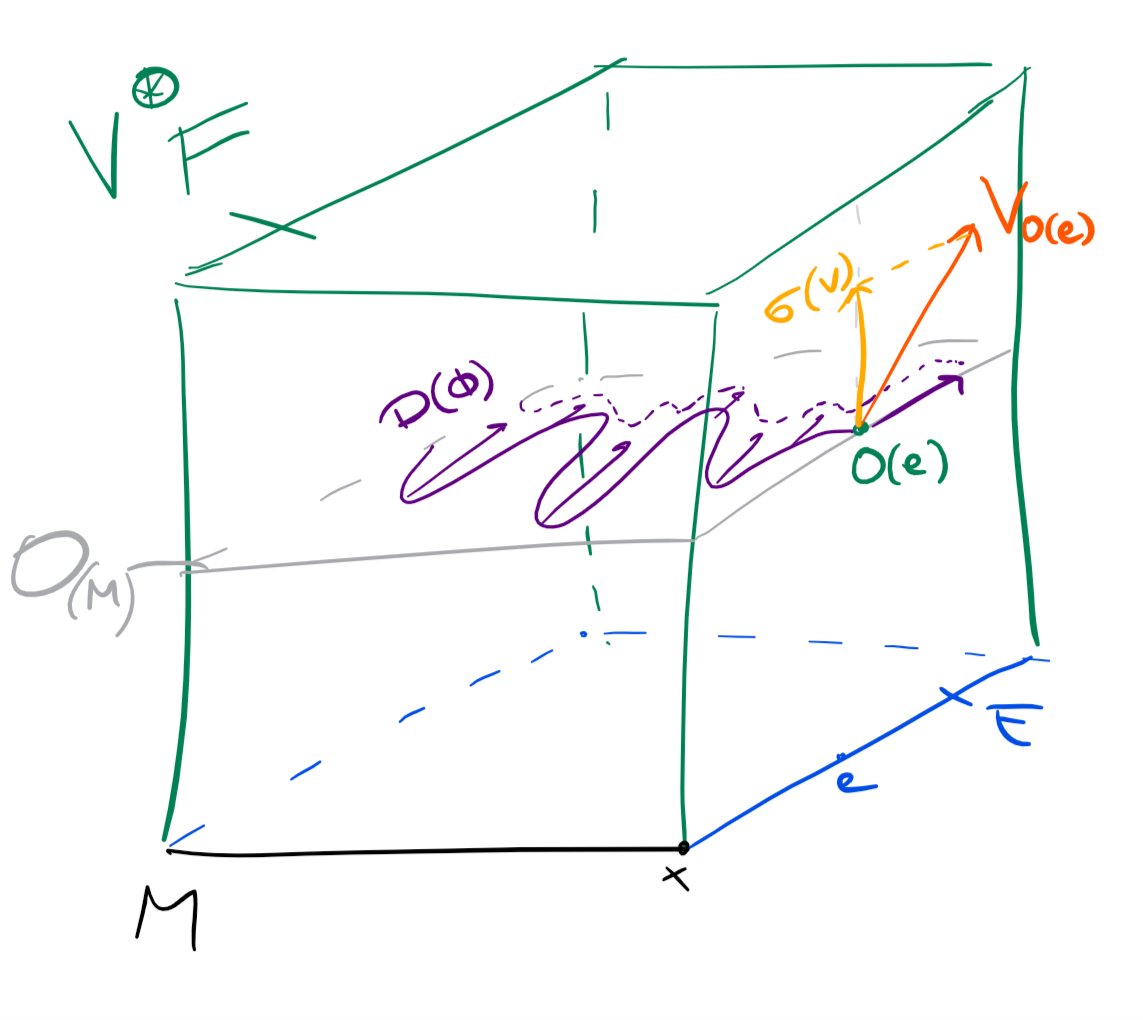
\includegraphics{Pictures/fieldJacobi.png}
  \caption{.}
\end{figure}

\begin{figure}
  \centering
  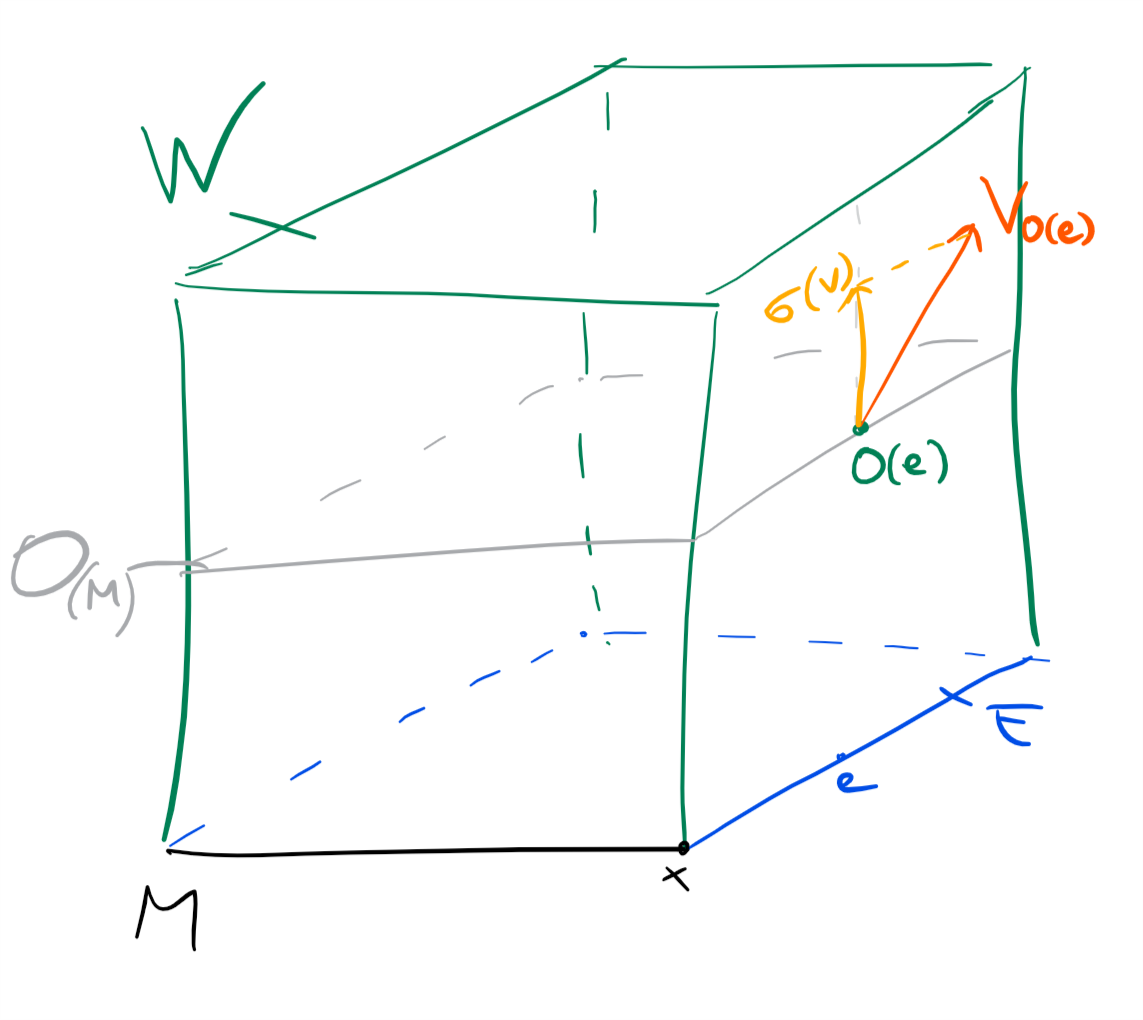
\includegraphics{Pictures/sigma.png}
  \caption{.}
\end{figure}

\begin{figure}
  \centering
  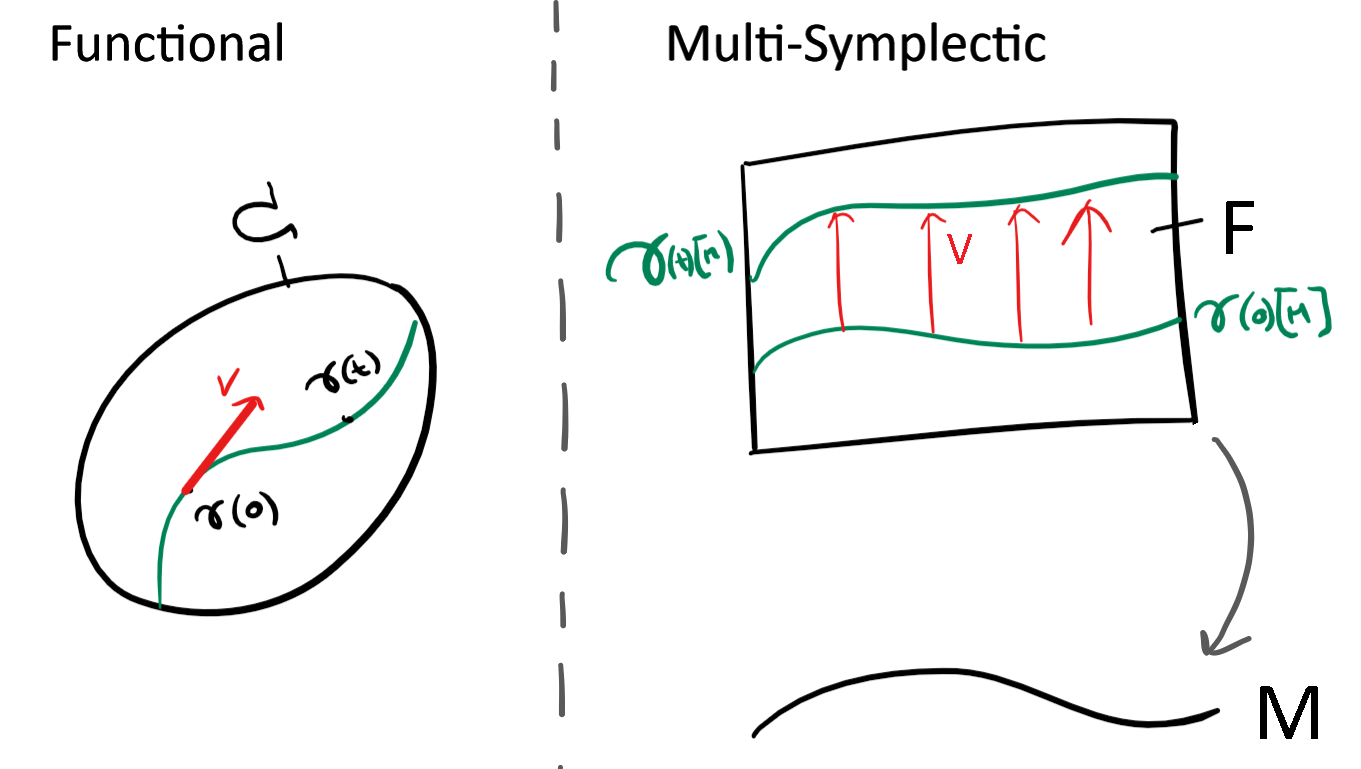
\includegraphics{Pictures/variations.png}
  \caption{.}
\end{figure}

%\bibliographystyle{abbrv}
%\bibliography{main}

\end{document}
